%Dokumentenklasse festlegen
\documentclass[11pt, a4paper, titlepage, oneside]{extarticle}

\usepackage[utf8]{inputenc}				%Deutsche Sprachanpassung
\usepackage[T1]{fontenc}                %Sibentrennung und Sonderzeichen
\usepackage[english]{babel}				%Eingabe der Sonderzeichen
\usepackage{cite}						%Für Literaturverzeichnis

\usepackage{eurosym}					%Eingabe von €-Zeichen

\usepackage{lmodern, fancyhdr}         	%Kopf-Fußzeile mit Gestaltungsmöglichkeit
\usepackage{graphicx, array}  			%einbinden von Grafiken
\usepackage{enumitem}
\usepackage{subfigure, tabularx}       	%besondere Gestaltungen bei Grafiken, erweiterte Tabellen
%\usepackage{lstlisting}
\usepackage{nameref}         		   	    	%zusätzliche referenzen zu sections
\usepackage[printonlyused, withpage]{acronym}
\usepackage{tablefootnote}
\usepackage{listings}                   		%Darstellung von Quellcode
\lstset{basicstyle=\footnotesize, captionpos=b}
\usepackage{lastpage}						%Lastpage

%Schrift global auf Helvetica umstellen
\renewcommand{\familydefault}{\sfdefault}
\usepackage{helvet} 
\usepackage{blindtext}

%\usepackage{array,booktabs,ragged2e}					%Tabellenalignment

%Raendereinstellung des Dokuments
\linespread{1.2}                         		%Zeilenabstand
\parindent0cm                            		%kein Zeileneinzug
\usepackage[left=30.00mm, right=20.00mm, top=30.00mm, bottom=30.00mm]{geometry}
\usepackage[pdftitle={Deployment}, 
            pdfsubject={Documentation}, 
            pdfauthor={3AAIF}, 
            pdfkeywords={Aufbaulehrgang, IT-Kolleg, Imst, Latex},
            colorlinks, 
            linkcolor=blue, 
            bookmarks, 
            bookmarksopen, 
            urlcolor=blue, 
            bookmarksnumbered, 
            final]{} 

%macros
%Makros festlegen
\newcommand\getDoctype{Documentation}
\newcommand\getMainTitle{Deployment}
\newcommand\getSubTitle{Seminar work}

\newcommand\getdm{Deployment}

\newcommand\getDeadline{XX.XX.XXXX}

\newcommand\getTeacher{Alexander Scharmer, BEd.}

\newcommand\getSchool{IT college Imst} 

\newcommand\getHeadofSchool{Dir. Dr. Stefan Walch}
\newcommand\getHeadGraphics{
\includegraphics[scale=0.6]{graphics/itkolleg_logo.pdf}}


\DeclareUnicodeCharacter{00A0}{ } 

\pagestyle{fancy}

%Kopfzeile
\lhead{\footnotesize \getSchool}
\chead{}
\rhead{\footnotesize \getMainTitle}


%Fußzeile
\lfoot{\footnotesize \getDoctype}
\cfoot{}
\rfoot{\footnotesize Page \thepage}

%Festlegung der Linie oben und unten
\renewcommand{\headrulewidth}{0.2pt}
\renewcommand{\footrulewidth}{0.2pt}

\begin{document}
	\pagestyle{empty}
	%Titelblatt
    \begin{titlepage}
  %\sffamily
    
    \vspace*{-2cm}     
    \begin{figure}[h]
        \centering
        \getHeadGraphics
    \end{figure}  
    
    \vspace{1cm}

    \begin{center}  
        %Haupttitel
        \huge{\textbf{\MakeUppercase{\getDoctype}}}
        \vspace{2cm}
    
        %erste Ueberschrift
        \LARGE{\getMainTitle} \\
		    \large{\getSubTitle} \\

    \end{center}
    
    \vfill
    
    This project was carried out by the students of the classes 3AAIF \& 3AKIF in the year of 2016.

\end{titlepage}
    
    %Inhaltsverzeichnis
    \thispagestyle{plain}

\newpage
\tableofcontents
   
    
    \pagestyle{fancy}
    
	%Projektdokumentation allgemein
        \newpage

    \setcounter{page}{1}          %Seitenzaehler auf = 1 setzen  
%    \shorthandoff{"}
    \section{Task Setting }
    
    \subsection{Initial Situation}
    ...
    
    \subsection{Project Goals}
    ...
    
    \vspace{.8cm}
	
	\textbf{Should Criteria}
	\begin{itemize}
	   \item ...
	\end{itemize}
     
     \textbf{Must Criteria}
     \begin{itemize}
     	\item ...
     \end{itemize}
     
	\subsection{Project Costs}
	...
	\subsection{Resources}
	A few resources used for organizational and technical reasons:
	\begin{itemize}
		\item GitLab
		\item Dropbox
	\end{itemize}
	
	%\newpage
    \section{Realization}
	
    \subsection{Project Organization}
    
    
    \subsection{Leadership}
    \centering
    \begin{tabular}{rlr}
    	\hline 
    	\textbf{Deployment} & Theo Kapeller & 3AAIF \\ 
    	\hline 
    	\textbf{Virtualization} & Wolfgang Vitzthum & 3AAIF \\ 
    	\hline 
    	\textbf{Network} & Marco Schmid & 3AKIF \\ 
    	\hline 
    \end{tabular}
    \flushleft
    
    \subsection{Participants}
    \begin{table}[h]
    	\centering
		\begin{tabular}{r|l}
			\textbf{Participant} & \textbf{Job} \\ 
			\hline 
			Dominik Holzmeister & File Server \\ 

			\hline 
			Maria Rasch & WSUS \\ 
			\hline 
			Markus Weissenbach & DNS \\ 
			\hline 
			Simon Nagele & Network \\ 
			\hline 
			Elias Gabl & DNS \\ 
			\hline 
			Ludwig Thoma & DHCP \\ 
			\hline 
			Sebastian Tratter & Backup \\ 
			\hline 
			Thomas Streitberger & AD DS \\ 
			\hline 
			Marco Schmid & Network \\ 
			\hline 
			Dominik Kostenzer & ADK \& SQLexpress \\ 
			\hline 
			Theo Kapeller & ADK \& SQLexpress \\ 
			\hline 
			Wolfgang Vitzthum & Virtualization \\ 
			\hline 
			Lukas Oberhofer & Virtualization \\ 
			\hline 
			Marino Buljubasic & DHCP \\ 
			\hline 
			Christian Löw & Virtualization \\ 
			\hline 
			Benedikt Mayr & Virtualization \\ 
			\hline 
			Peter Pollheimer & Designation Conventions \& Documentation \\ 
			\hline 
			Jakob Tomasi & Documentation \\ 
			\hline 
			Dominik Perfler & Git-Human \\ 
			\hline 
		\end{tabular}
	\end{table}
    
    %Virtualisierungsmoegichkeiten
    \newpage

\section{Virtualization}

\subsection{Definition}

Wikipeadia defines virtualization as follows:
\\In computing, virtualization refers to the act of creating a virtual (rather than actual) version of something, including virtual computer hardware platforms, operating systems, storage devices, and computer network resources. \\
Source: https://en.wikipedia.org/wiki/Virtualization

\subsection{Types of virtualization}

\subsubsection{Server virtualization}

The virtualization of servers is using the virtualization of computers which is also called hardware- or para-virtualization. By using this method a special operation system called "hypervisor" needs to be installed on physical hardware. The hypervisor is responsible for managing the physically available resources of the host computer, like CPU, RAM, storage and ports. By doing this, the hardware used by virtual operating systems is depending on the host computer (hypervisor).

\subsubsection{Desktop virtualization}

The virtualization of desktop PCs is technically identical with the server-virtualization technique. The newest generation of desktop virtualization is able to stream a virtual PC onto the users devices (notebook, tables, thin clients). This is often used by owning a centralized large-scale physical server, which provides the operating systems for all clients connected to it.
\newline
\newline
Template for the virtual network boot client is \underline{THC0001}.

\subsubsection{Application virtualization}

The virtualization of an application allows to easily deploy software packages to a users device (PC, Notebooks, Tablets etc.). This is done by creating and copying a excutable ".exe" file to a shared network folder. By storing the file on the network, the installation and configuration is only done once. Available software products for this purpose are VMware ThinApp and Spoon Virtual Application.

\subsubsection{Type 1 virtualization}

Type 1 hypervisors run directly on the system hardware. They are often referred to as a "native" or "bare metal" or "embedded" hypervisors in vendor literature.
\\
Source: http://searchservervirtualization.techtarget.com/feature/Whats-the-difference-between-Type-1-and-Type-2-hypervisors

\subsubsection{Type 2 virtualization}

Type 2 hypervisors run on a host operating system. When the virtualization movement first began to take off, Type 2 hypervisors were most popular. Administrators could buy the software and install it on a server they already had.
\\
Source: http://searchservervirtualization.techtarget.com/feature/Whats-the-difference-between-Type-1-and-Type-2-hypervisors

Source: http://searchservervirtualization.techtarget.com/feature/Whats-the-difference-between-Type-1-and-Type-2-hypervisors

\subsection{Products}

\begin{table}[h]
    \begin{tabular}{llll}
    ~                           & Proxmox VE           & VMware vSphere       & Windows Hyper-V                  \\ \hline
    Guest-OS-Support            & Windows, Linux (KVM) & Windows, Linux, UNIX & Modern Windows OS, limited Linux \\
    Open Source                 & Yes                   & No                 & No                             \\
    Linux Containers (LXC)      & Yes                   & No                 & No                             \\
    High availability           & Yes                   & Yes                   & Yes                               \\
    Live VM-Snapshots           & Yes                   & Yes                   & Yes                               \\
    Bare-metal-Hypervisor       & Yes                   & Yes                   & Yes                               \\
    Webinterface                & Yes                   & Yes                   & No                             \\
    Max. RAM and CPU for a Host & 160 CPU / 2 TB RAM   & 160 CPU / 2 TB RAM   & 64 CPU / 1 TB RAM                \\
    Pricing                     & Free               & Starting at 650,50EUR  & Free                             \\
    Support                     & Starting at 19,90/Month           & Starting at 257,79/Month    & Starting at 1.323,00/2Years \\
    \end{tabular}
\end{table}

    
    %Namenskonzepte
    \section{Designation Concepts}
\begin{lstlisting}[caption=Naming Convention,frame=single]  
Server<prefix><id>SRV001
Client<prefix><id>THC0001
Switch<prefix><id>SWT001
Drucker<prefix><id>PRT001
Router<prefix><id>RUT001
AccessPoint<prefix><id>ACP001
VoIP<prefix><id>VIP0001
Firewall<prefix><id>VFW001
\end{lstlisting}
\newpage

\subsection{Server roles}
\begin{table}[h]		
	\begin{tabular}{l|l}
		\textbf{Server} & \textbf{Role}                                        \\ \hline
		SRV110          & DC, ADDS, DNS ,DHCP, WDS (PXE)                       \\ 
		SRV111          & MDT, ADK, MDT Workbench 2013, SQL Express, WSUS/WIDS
	\end{tabular}
	\caption{Server roles}
	\label{Tbl_Server_roles}
\end{table}

\subsection{Passwords and Logins}
\begin{table}[h]
	\begin{tabular}{l|l|l|l}
		\textbf{Machine}             & \textbf{Password}   & \textbf{Login}         & \textbf{Email}            \\ \hline
		Proxmox             & 12345      & root          & mail@example.org \\
		Windows Server 2012 & Password2! & Administrator & -                \\
		NAS Server			& 12345		 & admin		& -                 \\
		pfSense             & admin      & admin        & -                 \\
		Test client         & TestUser   & 1234         & -                 \\
	\end{tabular}
	\caption{Passwords and Logins}
	\label{Tbl_Passwords_Logins}
\end{table}

\subsection{Network Setup}
\begin{table}[h]	
	\begin{tabular}{l|l|l|l|l|l}
		\textbf{Name}         & \textbf{WAN} & \textbf{IP} & \textbf{Domain} & \textbf{Protocol} & \textbf{Ports Slaves}  \\ \hline
		Proxmox Network Setup & eth3         & 172.0.0.1   & test.lab        & LACP  			& eth1, eth2           
	\end{tabular}
	\caption{Network Setup}
	\label{Tbl_Network Setup}
\end{table}
\newpage



    
    %Netzwerk
    \section{Network Concepts}
\subsection{VLAN Network Convention}

\begin{table}[h]
	\begin{tabular}{lllll}
		\hline
		VLAN Name       & VLAN-ID & Net-Address       & Gateway         & Remarks      \\ \hline
		Board           & 10      & 192.168.10.0 /24  & 192.168.10.254  & Board only \\  
		Marketing       & 20      & 192.168.20.0 /24  & 192.168.20.254  & ~                           \\ 
		Production      & 30      & 192.168.30.0 /24  & 192.168.30.254  & ~                           \\ 
		WLAN Board      & 40      & 192.168.40.0 /24  & 192.168.40.254  & ~                           \\ 
		WLAN Employee   & 41      & 10.41.0.0 /16     & 10.41.255.254   & ~                           \\ 
		WLAN Guests     & 42      & 10.42.0.0 /16     & 10.42.255.254   & ~                           \\ 
		Virtual Servers & 50      & 192.168.50.0 /24  & 192.168.50.254  & ~                           \\ 
		Printer         & 60      & 192.168.60.0 /24  & 192.168.60.254  & ~                           \\ 
		VoIP            & 70      & 192.168.70.0 /24  & 192.168.70.254  & ~                           \\ 
		CCTV            & 80      & 192.168.80.0 /24  & 192.168.80.254  & ~                           \\ 
		NAS             & 90      & 192.168.90.0 /24  & 192.168.90.254  & ~                           \\
		Management      & 100     & 10.100.0.0 /16    & 10.100.255.254  & ~                           \\
		\hline
	\end{tabular}
	\caption{VLAN Convention}
	\label{Tbl_VLAN_Network_Convention}
\end{table}
    \input{13_network.tex}
    \input{14_DHCP.tex}
    \newpage


\section{Domain Network Service}

\subsection{Definition}

Wikipeadia defines DNS as follows:
he Domain Name System (DNS) is a system used to convert a computer's host name into an IP address on the Internet.



\subsection{Configuration DNS Server}



Gabl /Weissenbach\newline

We installed the Server-roll "DNS" on the (R010) Win 2012 Server.

Finally, start the DNS Manager under Tools / DNS in Server Manager.
There we have selected the point Reverse Lookupzonen and in the context menu the point New Zone. These settings were made individually for each Vlan.\newline


\begin{minipage}[X]{0.8\textwidth} 
	\centering 
		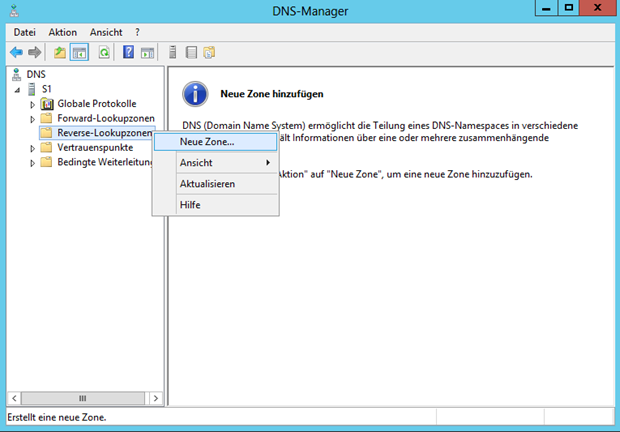
\includegraphics [scale=0.5]{graphics/1.png}
	\label{ecoconcept} 
\end{minipage} 
\newline\newline
We clicked through the welcome menu and selected Primary Zone.
\newline


\begin{minipage}[X]{0.8\textwidth} 
	\centering 
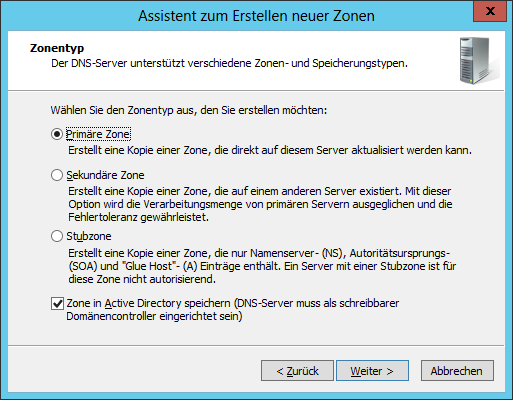
\includegraphics [scale=0.6]{graphics/2.png}
	\label{ecoconcept} 
\end{minipage} 


\begin{minipage}[X]{0.8\textwidth} 
	\centering 
	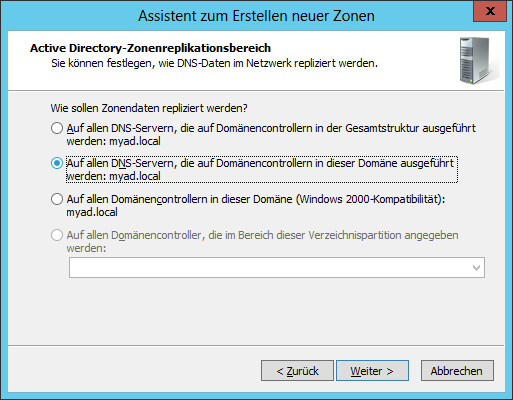
\includegraphics [scale=0.6]{graphics/3.png}	
	\label{ecoconcept} 
\end{minipage} \newline


Because it is an IPv4 network, we selected the IPv4 reverse lookup zone.\newline


\begin{minipage}[X]{0.8\textwidth} 
\centering 
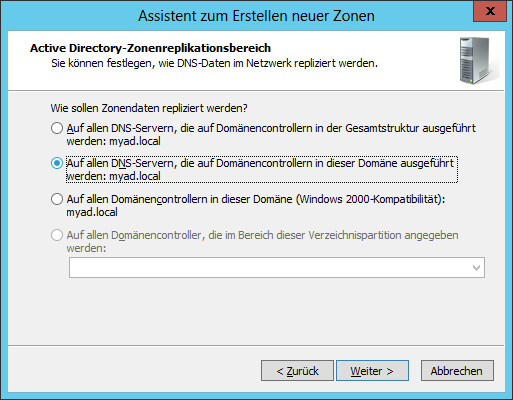
\includegraphics [scale=0.6]{graphics/4.png}
\label{ecoconcept} 
\end{minipage} \newline



Now we have specified the respective VLan. For this the fixed parts of the network address, as indicated in the screenshot.



We have retained the default setting for Dynamic Updates.\newline


\begin{minipage}[X]{0.8\textwidth} 
	\centering 
	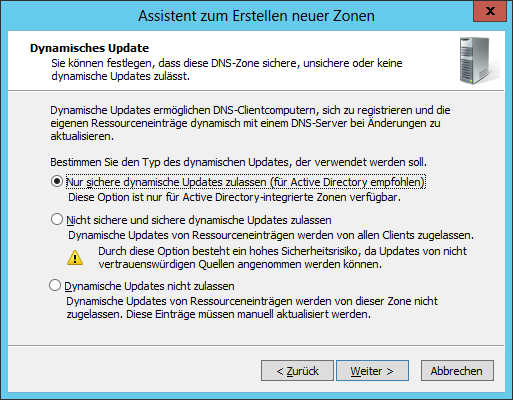
\includegraphics [scale=0.6]{graphics/5.png}
	\label{ecoconcept} 
\end{minipage} \newline

The DNS server, which is responsible for the respective VLAN, was informed of this. In order to resolve external addresses as well, a forwarding of the DNS queries must be created.\newline


\begin{minipage}[X]{0.8\textwidth} 
	\centering 
	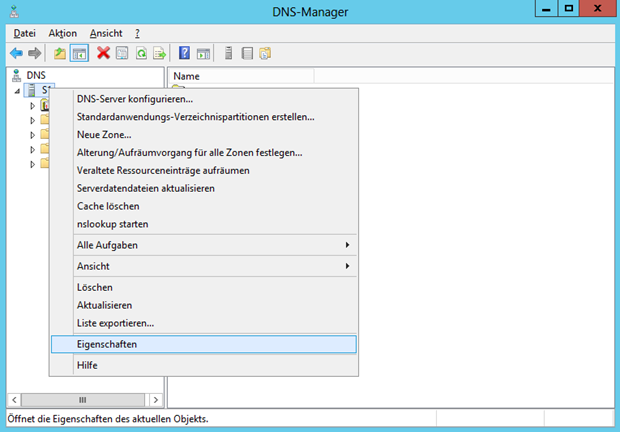
\includegraphics[scale=0.6]{graphics/6.png}  
	\label{ecoconcept} 
\end{minipage} \newline


In the IP settings of the clients on the network, the DNS server must be entered as the primary DNS server.\newline

    
    %Windows Server
    \input{16_Windows_Server.tex}
    \input{17_Active_Directory.tex}
    \input{18_Backup.tex}
    
    %Deployment
    \newpage
\input{deployment/141_dhcp.tex}
\newpage
\input{deployment/142_dns.tex}
\newpage
\input{deployment/143_fileserver.tex}
\newpage
\input{deployment/144_backup.tex}
\newpage
\input{deployment/145_usermanagement.tex}
\newpage
\input{deployment/146_securitypolicies.tex}
    
    %Begriffserklärung
    %\newpage
    %\section{Glossary}
\subsection{MySQL}
MySQL is an open source database management system (DBMS). It is in use on more than 50 million implementations\footnote{state 2013} and thus the most used DBMS in the world.

\subsection{XAMPP}
Damit MySQL seine Daten speichern kann, wird ein MySQL-Server benötigt. Dafür gibt es eine Open-Source Software die den Namen XAMPP trägt. XAMPP kann von der offiziellen Webseite\footnote{https://www.apachefriends.org/de/index.html} heruntergeladen werden und wird dann auf dem Rechner installiert. In der folgenden Abbildung kann man die Benutzeroberfläche von XAMPP sehr gut erkennen und den aktiven MySQL-Server.

\subsection{Navicat}
Um eine Verbindung mit der Datenbank herzustellen  hat sich das Team des HTL Eventmanager für die Open-Source Software Navicat Lite von der Firma PremiumSoft entschieden. Das Programm wird kostenlos von der offiziellen Homepage\footnote{http://www.navicat.com/} heruntergeladen und dann auf dem Rechner installiert. Navicat ist eine optisch top gestaltete Software für die Verwaltung von Datenbankverwaltungssystemen. Der Umgang mit Navicat ist sehr einfach gehalten und schnell anzulernen.

     
     \subsection{Responsive Webdesign}
     Responsive Webdesign (kurz RWD) bezeichnet ein gestalterisches Paradigma zur Entwicklung von Webseiten. Wurde eine Webseite "responsive" entwickelt, passen sich Elemente wie Navigation, Texte, Bilder, Seitenspalten, etc. an die Eigenschaften des Darstellungsgerätes (bspw. Bildschirmbreite und -Auflösung) an und erlauben dadurch eine korrekte Darstellung , egal ob Desktop, Smartphone oder Tablet.\\
     Die Site gewinnt an Übersichtlichkeit und der Nutzer ist nicht mehr gezwungen, horizontal zu scrollen und kann dadurch die Webseite komfortabel nutzen.
     
     \subsection{Hypertext Markup Language}
     Die Hypertext Markup Language (kurz HTML) ist eine textbasierte Auszeichnungssprache zur Definition von Seitenstrukturen wie Texten, Bildern, Links und Aufbauelemente. HTML stellt die Grundlage des World Wide Web dar und wird vom WWW Consortium (W3C) und der Web Hypertext Application Technology Working Group (WHATWG) weiterentwickelt.\\
     Für den \getHauptTitel wird die aktuellste Version HTML5 verwendet.
     
     \subsection{JavaScript}
     JavaScript wurde entwickelt um HTML-Seiten zu dynamisieren. Ferner wurde eine Skriptsprache entworfen, mit der es möglich ist, Benutzerinteraktionen auszuwerten, Inhalte zu verändern und so die Potentiale von HTML und CSS zu erweitern. Damit JavaScript funktioniert, muss der verwendete Browser über einen JS-Interpreter verfügen. Heutzutage ist das die Norm, es kann jedoch vorkommen dass JS aus Sicherheitsgründen deaktiviert wurde.
     
     \subsection{Document Object Model}
     Das Document Object Model DOM ist eine Schnittstelle für den Zugriff auf HTML-Dokumente. Sie erlaubt z.B. mit JavaScript dynamisch Inhalte, Strukturen und Layouts zu manipulieren. Vor der Entwicklung von DOM in den 90ern konnte auf HTML-Dokumente nur rudimentär mit JavaScript zugegriffen werden. Die meisten Browserhersteller entwickelten hierfür eigenständige Modelle. Dadurch entstand für Webentwickler die Notwendigkeit, für jeden zu unterstützenden Browser eine eigens angepasste Version zu schreiben. Die ersten vom W3C entwickelten DOM-Standards galten daher der Zusammenführung und Standardisierung des dynamischen Zugriffs auf HTML-Dokumente.
     
     \subsection{Cascading Style Sheets}
     CSS, verwendet in der Version 3, ist eine Gestaltungssprache für HTML und DOM-Objekte. Mit Hilfe von Selektoren kann auf Objekte zugegriffen werden um diese grafisch anzupassen. Hierfür bietet CSS etliche Anweisungen für Dimensionierung, Farbgestaltung, Animierung, Schrifttypen, etc. pp.

	\subsection{Font}
	Als Font bezeichnet man die elektronische Form einer Schriftart. Diese werden zur Darstellung von Zeichenketten auf Bildschirmen oder für die Ausgabe am Drucker verwendet. Man unterscheidet in zwei Kategorien, basierend auf der Art der Speicherung, welche entweder raster- oder vektorbasiert in einer Fonts-Datei (.tff) erfolgt.
	Während bei einer Rasterspeicherung jedes Pixel einer sogenannten Glyphe einzeln festgelegt ist, werden für Vektorenfonts nur mathematische Angaben der Umrisse abgespeichert.
	
	\lstset{frame=shadowbox, breaklines=true}

	\subsection{World Wide Web Consortium (W3C)}
		Beim World Wide Web Consortium handelt es sich um das Gremium für die Standardisierung aller wichtigen Internettechniken die maßgeblich für das Surfen im Internet (dem World Wide Web) sind.
		Die W3C gibt vor, wie gültiger HTML-, XML- oder auch CSS-Code auszusehen hat.
		Browserhersteller und Webprogrammierer sollten sich an diese Standards halten um eine fehlerfreie Darstellung zu garantieren. Die Identifizierung eines Standards innerhalb eines HTML-Dokumentes erfolgt mithilfe von sogenannten Doctypes.\\
		Diese müssen zwingend in der ersten Zeile eines HTML-Dokumentes definiert werden.
	
	\begin{lstlisting}
	<!DOCTYPE HTML PUBLIC "-//W3C//DTD HTML 4.01//EN"
	"http://www.w3.org/TR/html4/strict.dtd">
	\end{lstlisting}
		Der Dokumententyp eines HTML 4.01 Dokumentes mit Verweis zur W3C-Spezifikation.\\
	
	\begin{lstlisting}
	<!DOCTYPE html>
	\end{lstlisting}
		Der Dokumententyp eines HTML 5 Dokumentes. Mit HTML 5 entfallen erstmals die Querverweise zur W3C.
		
	\subsection{Daemon}
		Ein Daemon wird unter Linuxumgebungen ein Hintergrundservice genannt der permanent läuft und keine Interaktion mit dem Benutzer benötigt.
		Ein Daemon wird meistens durch ein "d" am Ende seines Namens gekennzeichnet.\\
		Beispiele für Daemons sind der Apache Webserver (httpd), der MySQL Server (mysqld) oder auch der SSH Server (sshd).
		
	\subsection{SQL Injections}
		SQL Injections sind Attacken welche probieren SQL-Code in eine SQL-Abfrage einzuschleusen.\\
		Bei nicht ausreichenden Sicherheitsvorkehrungen kann dies fatale Folgen für jeden Webdienst haben.\\
|"SELECT * FROM users WHERE firstname = ''; DROP TABLE users; -- '"|\\
		
		Durch eine Attacke wie diese kann unter anderem die komplette Datenbank ausgelesen, verändert oder sogar gelöscht werden.
	
	\subsection{Captcha}
		Bei Captchas handelt es sich um kleine Bilder welche authentische Benutzer von Bots unterscheiden sollen.
		Erreicht wird dies oft durch verschwommene oder verschobene Buchstaben und Zahlenkombinationen welche darauf abzielen nur von Menschen identifiziert zu werden.
	
		
		Captchas sind vorallem wegen der Unlesbarkeit für ältere Menschen und Menschen mit Sehschwächen bekannt sowie für die recht leichte Erkennung einiger Captchas durch Computerprogramme.
		
	\subsection{Timestamp}
		Ein Timestamp (auch Unixzeit genannt) bildet die Zeit in Sekunden ab, welche seit dem 1. Januar 1970 um 00:00 Uhr (UTC) vergangen sind.
		Dieser Timestamp erleichtert die Arbeit mit Zeitpunkten ungemein da ein Zeitstempel unabhängig von Zeitzonen sowie Sommer- und Winterzeit berechnet wird.\\
		
		Beispiel: Der \textbf{15. Februar 2015 um 17:26:25} entspricht einem Timestamp von \textbf{1424017585}.\\
		
		Die 32-Bit Zeitstempel, welche vorallem in alten Betriebssystem verwendet werden, erreichen am 19. Januar 2038 ihr Limit und sind ab diesem Zeitpunkt nicht mehr einsatzfähig.
	
    
    %Abbildungsverzeichnis
    \newpage
    \listoffigures
    
    %Tabellenverzeichnis
    \newpage
    \listoftables
    
    %Quellenverzeichnis
    \newpage
    \begin{Large}
\textbf{Literature/Sources}
\end{Large}

\textbf{TODO: implement package for literature management}
\end{document}
